\documentclass[onecolumn]{article}
\usepackage{graphicx}

\begin{document}

\title{Determine the smallest circle enclosing a set of points}

\author{Arjen Markus}

\maketitle


\subsection*{Introduction}

A simple problem in computer graphics is to determine the bounding box that encloses a set of points
or more generally, any set of graphical objects. You simply scan the objects' coordinates, take the minimum
and maximum x-coordinates, the minimum and maximum y-coordinates and there you are: the coordinates of the
bounding box. This is so simple because the sides of such a box are aligned with the coordinate axes.

Things become more complicated when you want to know the smallest rectangle of whatever orientation around
these objects. One small complication is: what do yu mean by smallest rectangle? It could the one with the
smallest sides -- then you would probably end with a square -- or the smallest surface area or the smallest
circumference. These are minor issues, perhaps, but still important as you will want to make the meaning precise.

Here we concentrate on a circle. As it has only one size parameter, the radius, this definition difficulty does
not show up. But determining the smallest circle is not entirely trivial. The first step is to find out which
two points are furthest away from each other. This will tell us the \emph{minimum} radius that can at all work.
It may not be the radius of the smallest circle that contains all points though.

\begin{figure}[h]
\begin{center}
\caption{Illustration of the candidate circle. The grey area may also contain points, in which case the
circle needs to be enlarged.}
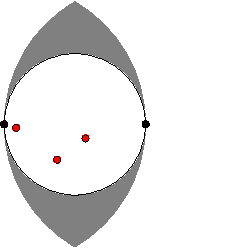
\includegraphics[width=0.7\textwidth]{candidate_circle.pdf}
\label{candidate}
\end{center}
\end{figure}

\subsection*{A candidate circle}
Take the set of points in figure \ref{candidate}. We have a circle of radius $R$ that connects the two points that
are furthest apart and we have two circles around these two points with a radius $2R$ to indicate the area wher
we should find all points of our point set. If there are points in the grey area, they lie outside the
circle that is one candidate for the smallest circle, so then we need a larger circle still.

\subsection*{A larger circle}
Suppose we have a point near the top of the grey area, like in figure \ref{point_outside}. This would be at a distance $R$
from the two points that determine the candidate circle, and so form a equilateral triangle. The thin black circle
shows which points are at a distance R or less from this new point.

The smallest circle that will enclose the point (lightblue), the two points from the candidate circle and the two
valid points inside it, has a radius $r$ determined by the equilateral triangle. The side of the triangle is equal to $2R$.
Some straightforward algebra and geometry leads to:

\begin{equation}
    r = \frac{2}{3} \sqrt{3} R \approx 1.1545 R
\end{equation}

This is likely to be the upper limit for the smallest circle around a set of points. If the points in the grey
area are closer to the candidate circle, then the smallest circle will be determined by the triple of points giving
the smallest circumcircle. Which three points that would be, remains to be seen. An obvious method would be to simply
try them all, but since the difference is fairly small, a reasonable approxmate method would be:
\begin{itemize}
\item
Determine the two points with the largest distance $2R$ to each other. This gives the candicate circle.
\item
If all points lie in there or on the circumference, we are done.
\item
Otherwise take the circle with radius $\frac{2}{3} \sqrt{3} R$ that passes through these two points and either of the
extreme points in the grey area.
\end{itemize}

While it is an approximation, you would make an error in the radius of at most 15\% and the method uses
$O(N^2)$ operations instead of $O(N^3)$ if you were to examine all possible circumcircles.

TODO:

How to determine such a larger circle that does enclose all points (though not perfectly)?

\begin{figure}[h]
\begin{center}
\caption{Situation with an additional point in the grey area. The lowest of the points inside the candidate
should be removed, as it is at a greater distance from the lightblue point than R.\\
}
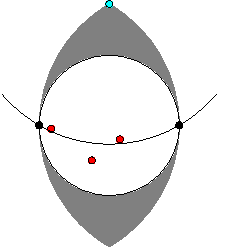
\includegraphics[width=0.7\textwidth]{point_outside.pdf}
\label{point_outside}
\end{center}
\end{figure}

\end{document}
